% !TeX program = xelatex
% 混凝土骨料颗粒智能筛分比拼 — 答辩 PPT（自然堆积赛道）
% 编译: latexmk -xelatex main.tex  或  make
% 引擎: XeLaTeX + ctexbeamer + aspectratio=169

\documentclass[UTF8,aspectratio=169,12pt]{ctexbeamer}

\usetheme{Madrid}
\usecolortheme{default}
\setbeamertemplate{navigation symbols}{}
\setbeamertemplate{footline}[frame number]

% --- 字体与图形 ---
\usepackage{graphicx}
\usepackage{tikz}
\usetikzlibrary{shapes,arrows,positioning}
\usepackage{booktabs}
\usepackage{amsmath}
\usepackage{hyperref}
\graphicspath{{figures/}{../../demo_data/samples/results/}{../../demo_data/samples/}{../paper/figures/}{../assets/}}

\title[骨料智能筛分（自然堆积）]{混凝土骨料颗粒智能筛分比拼}
\subtitle{自然堆积赛道：Cellpose-SAM $\to$ 质量加权筛分}
\author[匿名]{匿名参赛队}
\date{2026年8月}
\institute[匿名]{}

\begin{document}

% --- 封面 ---
\begin{frame}
\titlepage
\begin{center}\small\textcolor{gray}{匿名评审：隐去学校、校徽、导师信息}\end{center}
\end{frame}

% --- 目录 ---
\begin{frame}{目录}
\tableofcontents
\end{frame}

\section{任务解读}

\begin{frame}{赛题：4 任务 + 4 评分维度}
\begin{columns}[T]
\begin{column}{0.58\textwidth}
\begin{itemize}\small
\item \textbf{任务1 精细识别}：粘连分离（颗粒 vs.\ 背景）
\item \textbf{任务2 粒径分析}：直径与 $D_{10}/D_{50}/D_{90}$
\item \textbf{任务3 形状分类}（加分）：针片／圆／棱角
\item \textbf{任务4 异常检测}：$>50$\,mm 异物／泥团
\end{itemize}
\vspace{0.4em}
{\scriptsize\textcolor{gray}{赛题见 \texttt{docs/task.md}；提交物见 \texttt{paper\_and\_slide.md}（PPT、代码、设备、技术报告）}}
\end{column}
\begin{column}{0.42\textwidth}
\begin{block}{评分（以筛分为准）}
\begin{itemize}\footnotesize
\item 粒径误差 40--50\% \textcolor{red}{主分}
\item 识别准确率 20--25\%
\item 算法创新性 15--20\%
\item 答辩表现 10--15\%
\end{itemize}
\end{block}
\vspace{0.4em}
\centering\small\textbf{现场 $\le 30$\,min，一键出报告}
\end{column}
\end{columns}
\end{frame}

\section{总体方案}

\begin{frame}{总体方案：4 步链（不改上游）}
\vspace{-0.2em}
\begin{center}
\begin{tikzpicture}[node distance=0.9cm, auto, scale=0.78, every node/.style={transform shape},
  block/.style={rectangle, draw, rounded corners, fill=blue!8, minimum height=0.88cm, minimum width=2.25cm, align=center, font=\footnotesize},
  arrow/.style={->, thick}]
\node[block] (img) {图像目录\\ \texttt{jpg/png}};
\node[block, right=0.95cm of img] (seg) {1.\ 分割\\ Cellpose-SAM};
\node[block, right=0.95cm of seg] (geo) {2.\ 几何\\ $b/a,\;A,\;P$};
\node[block, right=0.95cm of geo] (sieve) {3.\ 筛分等效\\ $d,w,D_{50}$};
\node[block, right=0.95cm of sieve] (rep) {4.\ 报告\\ \texttt{SceneSummary}};
\draw[arrow] (img) -- (seg); \draw[arrow] (seg) -- (geo); \draw[arrow] (geo) -- (sieve); \draw[arrow] (sieve) -- (rep);
\end{tikzpicture}
\end{center}
\vspace{0.4em}
\begin{table}\scriptsize
\begin{tabular}{p{2.9cm}p{3.8cm}p{5.3cm}}
\toprule
模块 & 关键产物 & 说明 \\
\midrule
\texttt{imagegrains} & \texttt{*\_pred.tif},\ \texttt{*\_grains.csv} & 预训练 \texttt{IG2\_full\_set\_cp\_SAM}（零样本） \\
\texttt{aggregate\_screening} & \texttt{*\_re\_scaled.csv} $\to$ 报告 & $d=\theta_{1}b+\theta_{2}d_{\mathrm{eq}}+\theta_{3},\ w=d^{\gamma}$ \\
\bottomrule
\end{tabular}
\end{table}
\vspace{0.2em}{\scriptsize\color{gray}{架构见 \texttt{docs/architecture.md}；数据流见 \texttt{data-flow.md}；质量加权是核心创新。}}
\end{frame}

\section{精细识别}

\begin{frame}{任务1 精细识别：Cellpose-SAM 粘连分离}
\begin{columns}[T]
\begin{column}{0.52\textwidth}
\begin{itemize}\footnotesize
\item 基座：ImageGrains 2.0 \texttt{IG2\_full\_set\_cp\_SAM}（Cellpose-SAM），IG2 多源多粒径，零样本泛化优于 YOLO/Mask R-CNN
\item 3 张样本：1924 / 968 / 966 颗粒，$3024\times4032$，$0.208$\,mm/px
\item 参数：\texttt{--diameter} 自适应，\texttt{--gpu} 真值，$2$--$3$\,s/张
\end{itemize}
\vspace{0.3em}
{\scriptsize\textcolor{gray}{左：原图\enspace|\enspace 中：掩膜\enspace|\enspace 右：叠加，可目检粘连与小颗粒召回}}
\end{column}
\begin{column}{0.48\textwidth}
\centering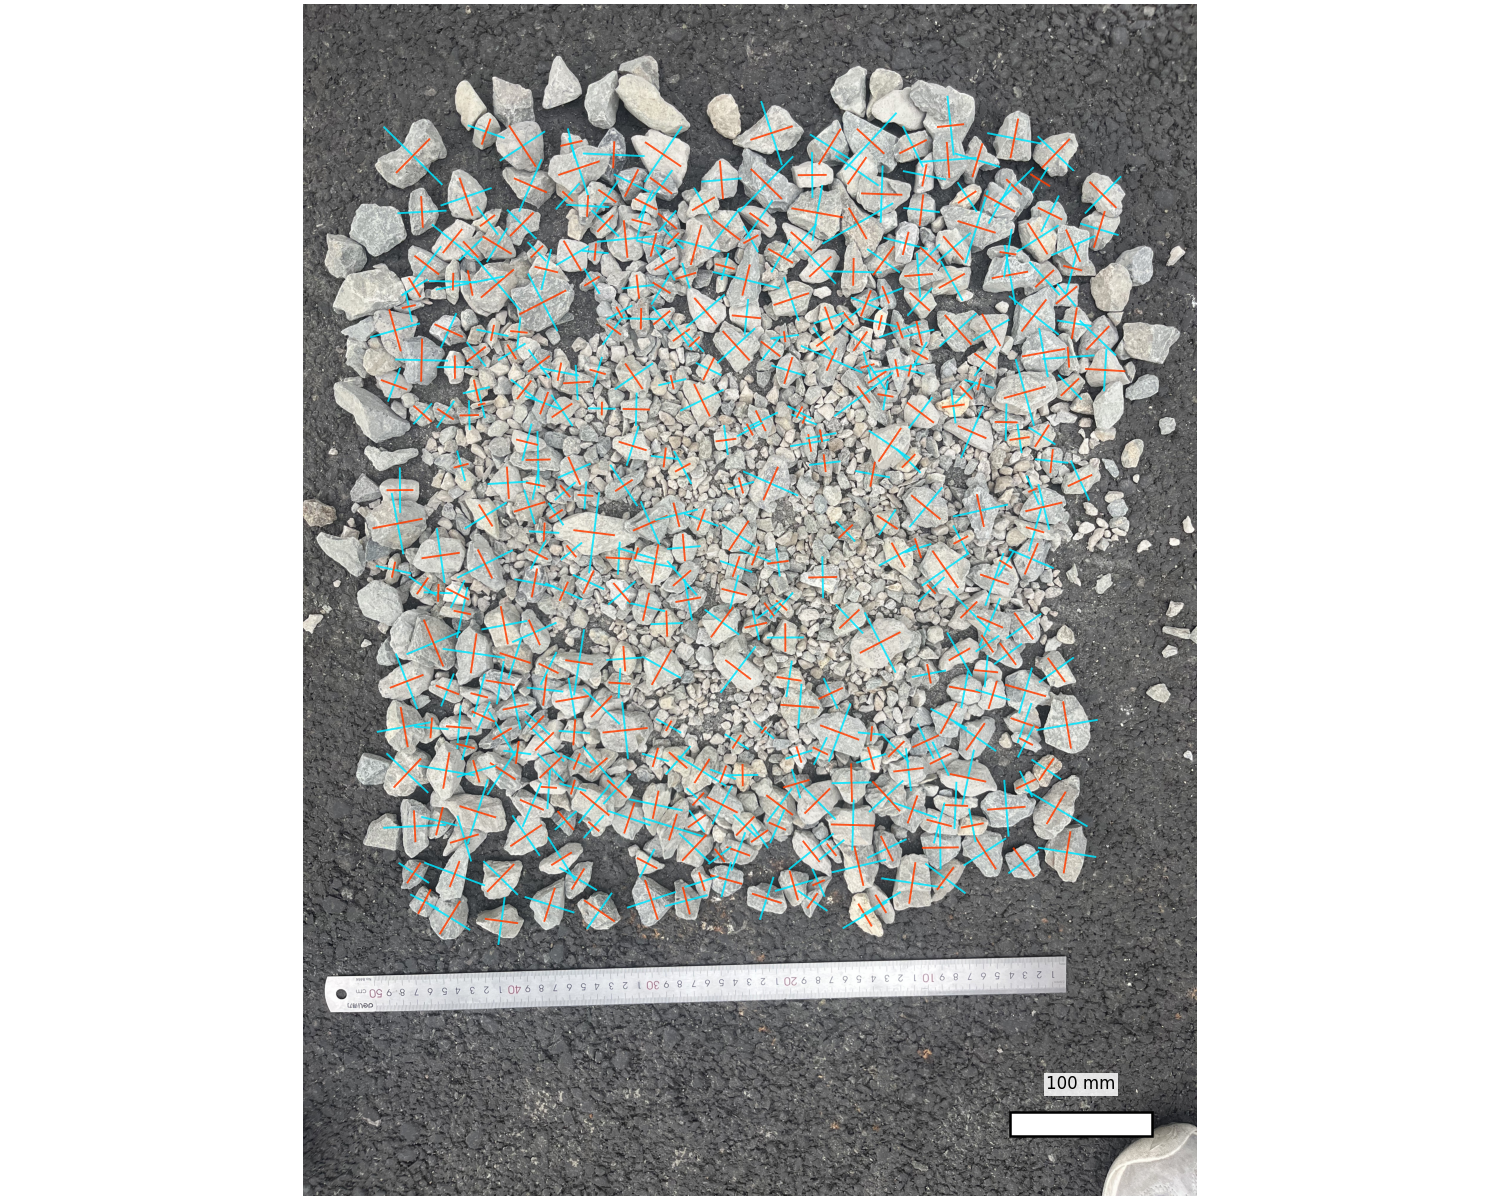
\includegraphics[width=\linewidth,height=3.6cm,keepaspectratio]{agg_001_IG2_full_set_cp_SAM_pred_grains_re_scaled_axes_overlay.png}\\
{\scriptsize\textcolor{gray}{示例：agg\_001 轴叠加（青 $a$／红 $b$，$n=1924$）}}
\end{column}
\end{columns}
\vspace{0.4em}
\begin{columns}
\begin{column}{0.32\textwidth}\centering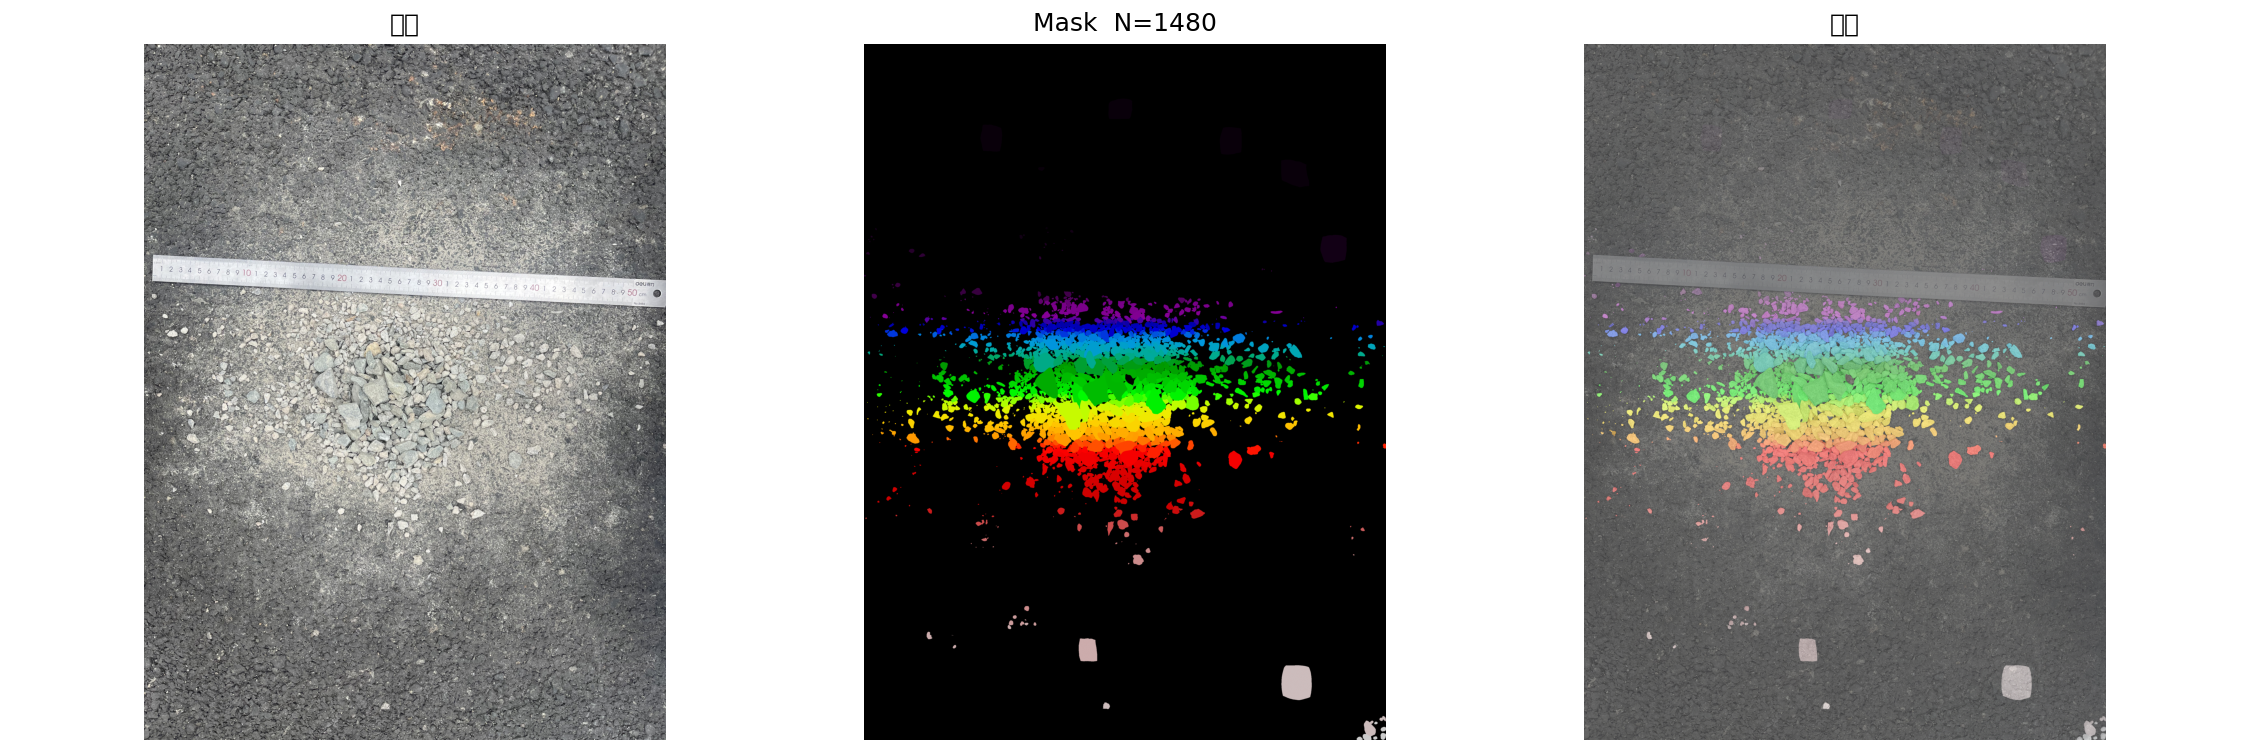
\includegraphics[width=\linewidth,height=2.3cm,keepaspectratio]{agg_029_IG2_full_set_cp_SAM_pred_grains_re_scaled_detection_overview.png}\\{\scriptsize agg\_029 细粒}\end{column}
\begin{column}{0.32\textwidth}\centering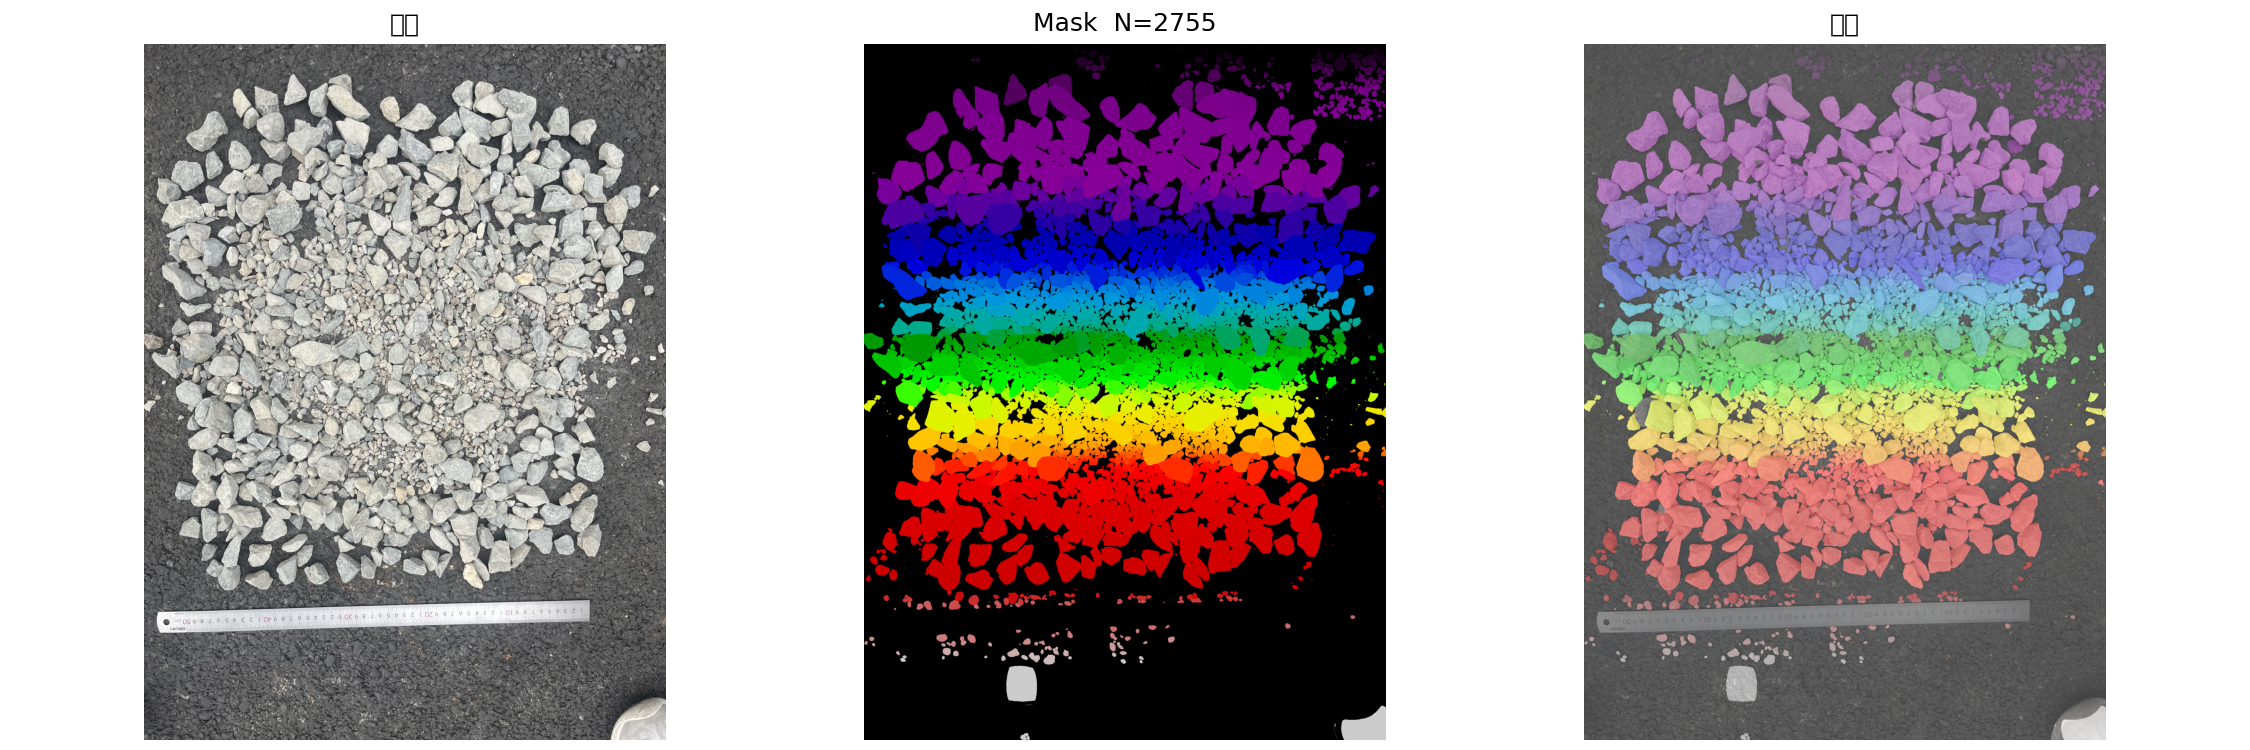
\includegraphics[width=\linewidth,height=2.3cm,keepaspectratio]{agg_001_IG2_full_set_cp_SAM_pred_grains_re_scaled_detection_overview.png}\\{\scriptsize agg\_001 中值}\end{column}
\begin{column}{0.32\textwidth}\centering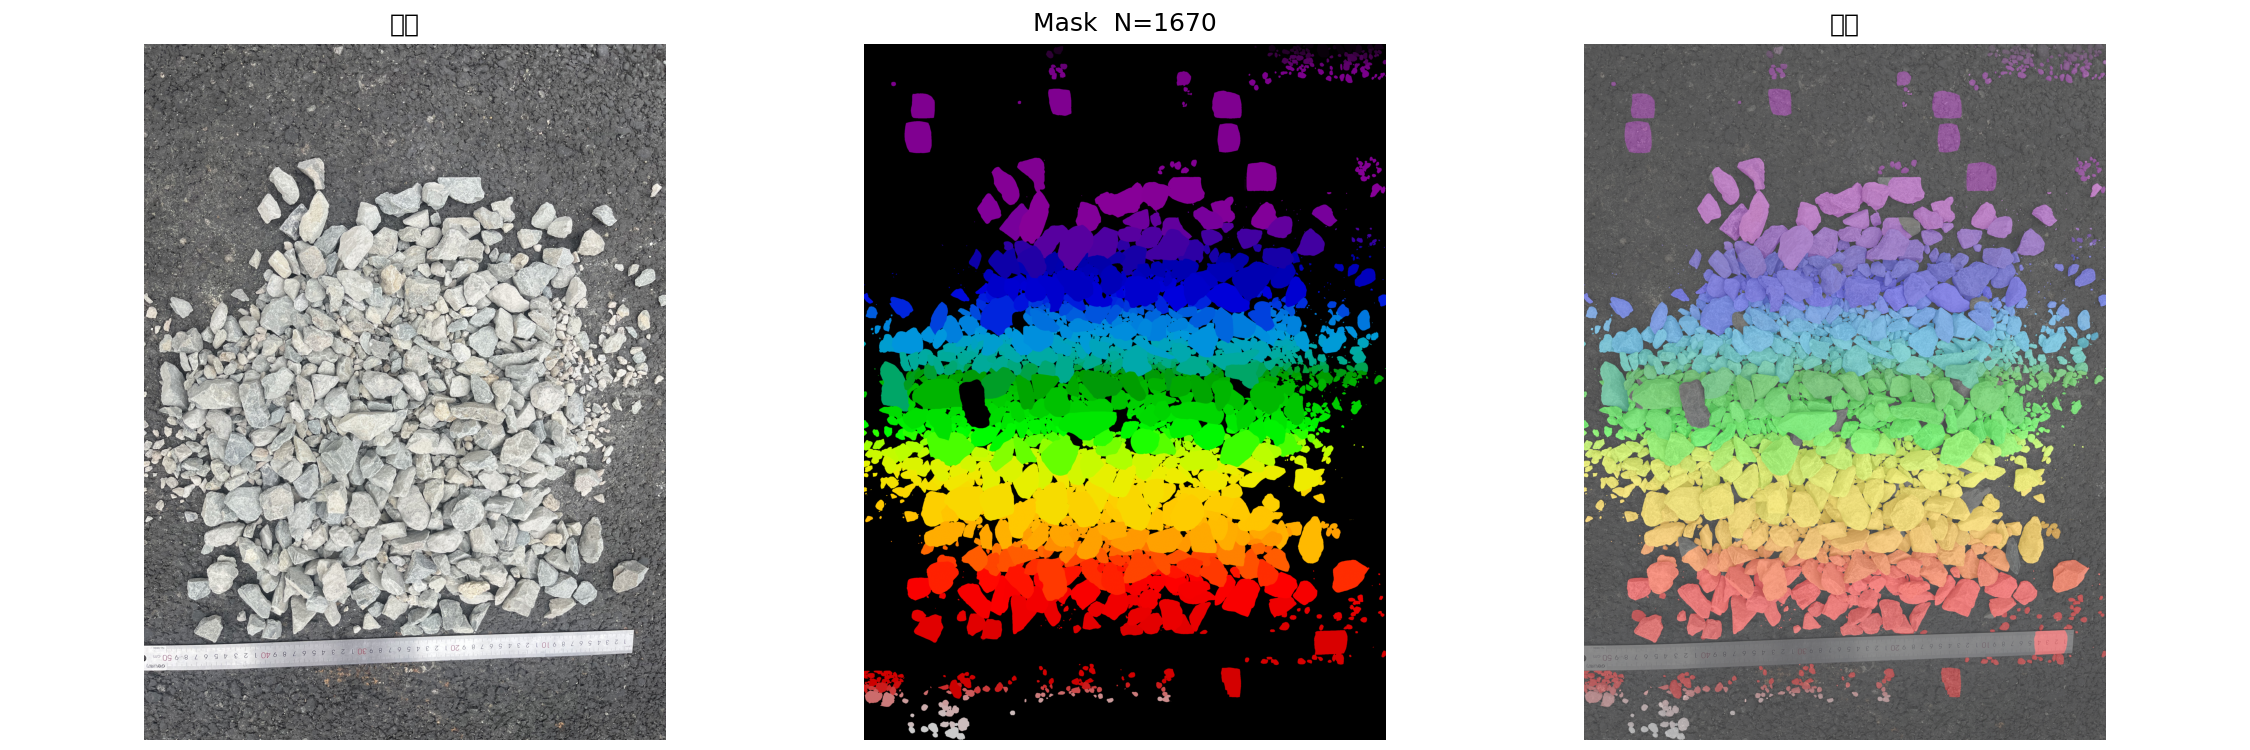
\includegraphics[width=\linewidth,height=2.3cm,keepaspectratio]{agg_005_IG2_full_set_cp_SAM_pred_grains_re_scaled_detection_overview.png}\\{\scriptsize agg\_005 粗粒}\end{column}
\end{columns}
\end{frame}

\section{粒径分析}

\begin{frame}{任务2 粒径分析：从像素到筛分语义}
\begin{columns}[T]
\begin{column}{0.53\textwidth}
\begin{itemize}\footnotesize
\item 几何：$b_{\mathrm{mm}}=b_{\mathrm{px}}\!\times\!\mathrm{res}$\\
\hspace{1em}$d_{\mathrm{eq}}=2\sqrt{A_{\mathrm{px}}\!\cdot\!\mathrm{res}^{2}/\pi}$
\item \textbf{质量加权}：$d=\theta_{1}b+\theta_{2}d_{\mathrm{eq}}+\theta_{3}$\\
\hspace{1em}$w=d^{\gamma}$\;($\gamma=3$ 体积)
\item 分位数：$D_{p}=F^{-1}(p)$\\
\hspace{1em}$F(d)=\sum w_{i}\mathbf{1}_{d_{i}\le d}/\sum w_{i}$
\item 双口径：数量 vs.\ 质量，\textbf{剔除后质量}为提交口径
\end{itemize}
\vspace{0.3em}
{\scriptsize
\begin{tabular}{lccc}
\toprule 样本 & 数量 $D_{50}$ & 质量 $D_{50}$ & 剔除后 \\
\midrule
agg\_029 & 5.2 & 14.1 & 14.6 \\
agg\_001 & 6.0 & 23.5 & 23.6 \\
agg\_005 & 7.6 & 27.5 & 27.5 \\
\bottomrule
\end{tabular}}
\end{column}
\begin{column}{0.47\textwidth}
\centering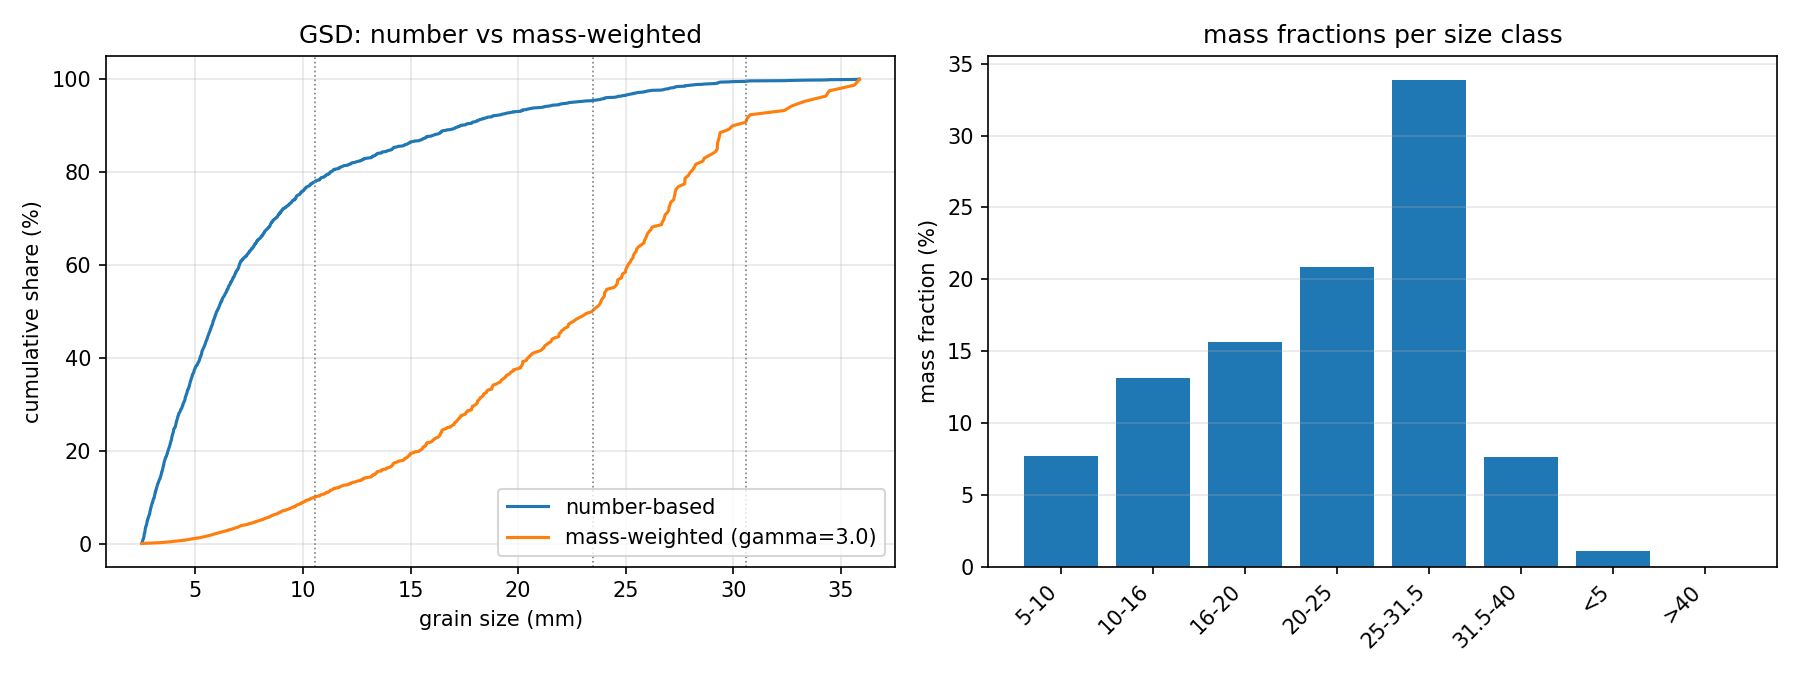
\includegraphics[width=\linewidth,height=3.8cm,keepaspectratio]{agg_001_IG2_full_set_cp_SAM_pred_grains_re_scaled_gsd_comparison.png}\\
{\scriptsize\textcolor{gray}{上：累计通过率（数量 vs.\ 质量）；下：粒级质量占比}}
\end{column}
\end{columns}
\end{frame}

\begin{frame}{粒径：长短轴可视化与校准}
\begin{columns}[T]
\begin{column}{0.52\textwidth}
\centering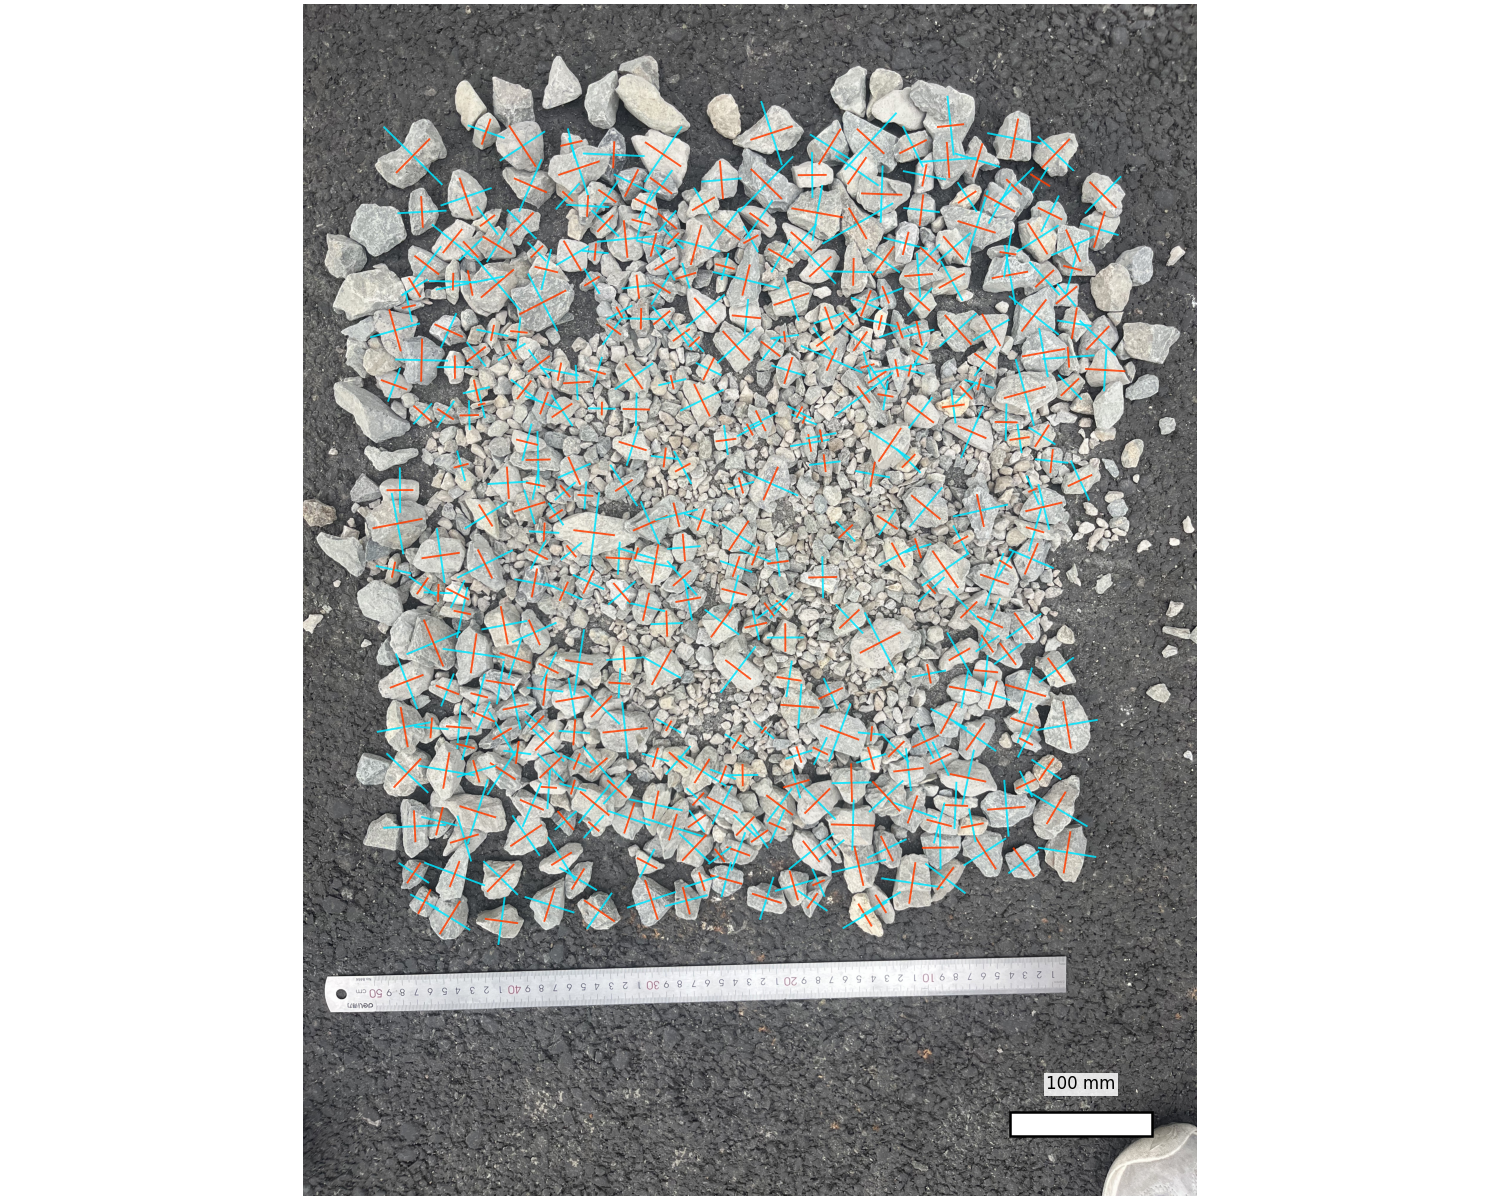
\includegraphics[width=\linewidth,height=4.2cm,keepaspectratio]{agg_001_IG2_full_set_cp_SAM_pred_grains_re_scaled_axes_overlay.png}\\
{\scriptsize 长短轴叠加（青 $a$／红 $b$）+ 右下比例尺（mm 可读）}
\end{column}
\begin{column}{0.48\textwidth}
\begin{block}{校准（需筛分真值）}
\footnotesize $\ge5$ 批：称重 $\to$ 筛分 $\to$ 拍照 $\to$ \texttt{fit\_calibration}（差分进化）得 $\theta,\gamma$，填 \texttt{--theta/--gamma}
\end{block}
\vspace{0.4em}
{\small 消融（agg\_001）：$\gamma=1\!\to\!3$ 时 $D_{50}$ $12.6\!\to\!23.7\!\to\!67.1$\,mm（含异物）$\to23.6$\,mm（剔除后），符合体积加权预期。}
\end{column}
\end{columns}
\end{frame}

\section{形状与异常}

\begin{frame}{任务3 形状分类 + 任务4 异常检测}
\begin{columns}[T]
\begin{column}{0.52\textwidth}
{\small\textbf{形貌}\;（$AR=b/a,\; C=4\pi A/P^{2},\; S=A/A_{\mathrm{convex}}$）：}
\begin{itemize}\footnotesize
\item 针片：$AR<0.5$
\item 圆形：$C>0.85\;\&\;S>0.95\;\&\;AR>0.8$
\item 棱角：$C<0.6$ 或 $S<0.9$
\item 优先级：棱角 $>$ 圆形 $>$ 针片 $>$ 普通
\end{itemize}
\vspace{0.2em}
{\scriptsize
\begin{tabular}{lcccc}
\toprule 样本 & 针片 & 圆形 & 棱角 & 普通 \\
\midrule
agg\_029 & 14.0 & 11.0 & 11.0 & 64.1 \\
agg\_001 & 16.3 & 8.0 & 16.4 & 59.3 \\
agg\_005 & 20.9 & 6.6 & 17.6 & 55.0 \\
\bottomrule
\end{tabular}}
\end{column}
\begin{column}{0.48\textwidth}
\centering

\includegraphics[width=0.47\linewidth,height=2.1cm,keepaspectratio]{agg_001_IG2_full_set_cp_SAM_pred_grains_re_scaled_shape_needle_flaky.png}\hfill

\includegraphics[width=0.47\linewidth,height=2.1cm,keepaspectratio]{agg_001_IG2_full_set_cp_SAM_pred_grains_re_scaled_shape_round.png}\\[0.25em]

\includegraphics[width=0.47\linewidth,height=2.1cm,keepaspectratio]{agg_001_IG2_full_set_cp_SAM_pred_grains_re_scaled_shape_angular.png}\hfill

\includegraphics[width=0.47\linewidth,height=2.1cm,keepaspectratio]{agg_001_IG2_full_set_cp_SAM_pred_grains_re_scaled_shape_regular.png}\\
{\scriptsize\textcolor{gray}{四类高亮（agg\_001，$n=1924$）}}
\end{column}
\end{columns}
\vspace{0.3em}
\centering{\scriptsize\textbf{异常}：$>50$\,mm 异物／$<5$\,mm 噪声／$40$--$50$\,mm $\&$ $S<0.85$ 泥团；3 样本均无泥团/异物，噪声 $27$--$46\%$（数量占比高，\mbox{质量权重低}）。}
\end{frame}

\section{实验验证}

\begin{frame}{实验验证：3 样本覆盖细／中／粗}
\begin{table}\scriptsize
\begin{tabular}{lcccccc}
\toprule 样本 & $n$ & $n_{\mathrm{normal}}$ & $D_{10}$ & $D_{50}$ & $D_{90}$ & 主粒级 \\
\midrule
agg\_029 & 966 & 520 & 6.7 & 14.6 & 30.6 & $5$--$10$\,($32.7\%$) \\
agg\_001 & 1924 & 1193 & 11.1 & 23.6 & 30.6 & $25$--$31.5$\,($34.2\%$) \\
agg\_005 & 968 & 703 & 15.6 & 27.5 & 38.0 & $25$--$31.5$\,($29.7\%$) \\
\bottomrule
\end{tabular}
\end{table}
\vspace{0.3em}
\begin{columns}
\begin{column}{0.32\textwidth}\centering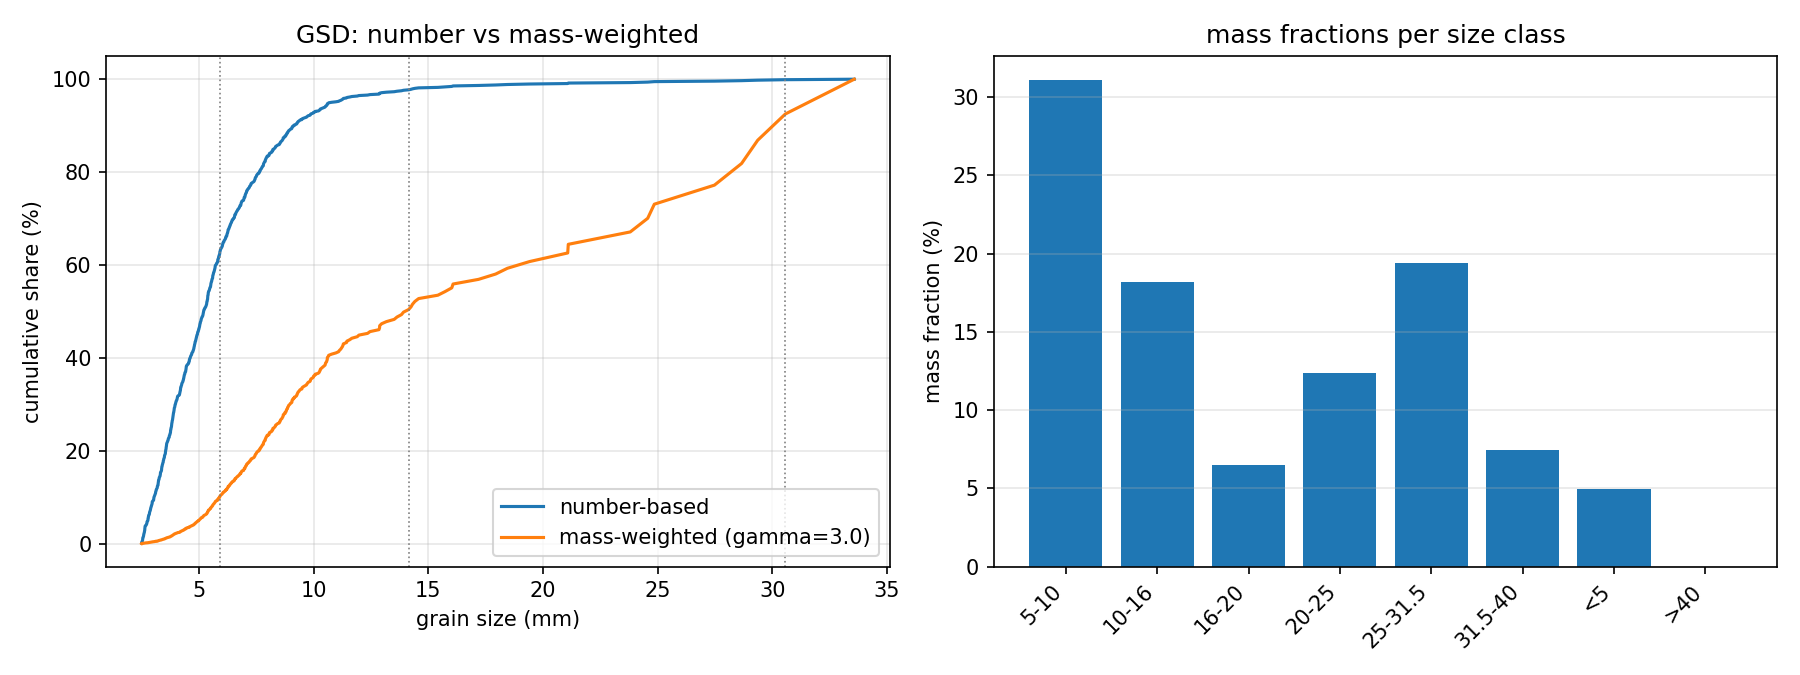
\includegraphics[width=\linewidth,height=2.6cm,keepaspectratio]{agg_029_IG2_full_set_cp_SAM_pred_grains_re_scaled_gsd_comparison.png}\\{\scriptsize 细粒：$D_{50}=14.6$}\end{column}
\begin{column}{0.32\textwidth}\centering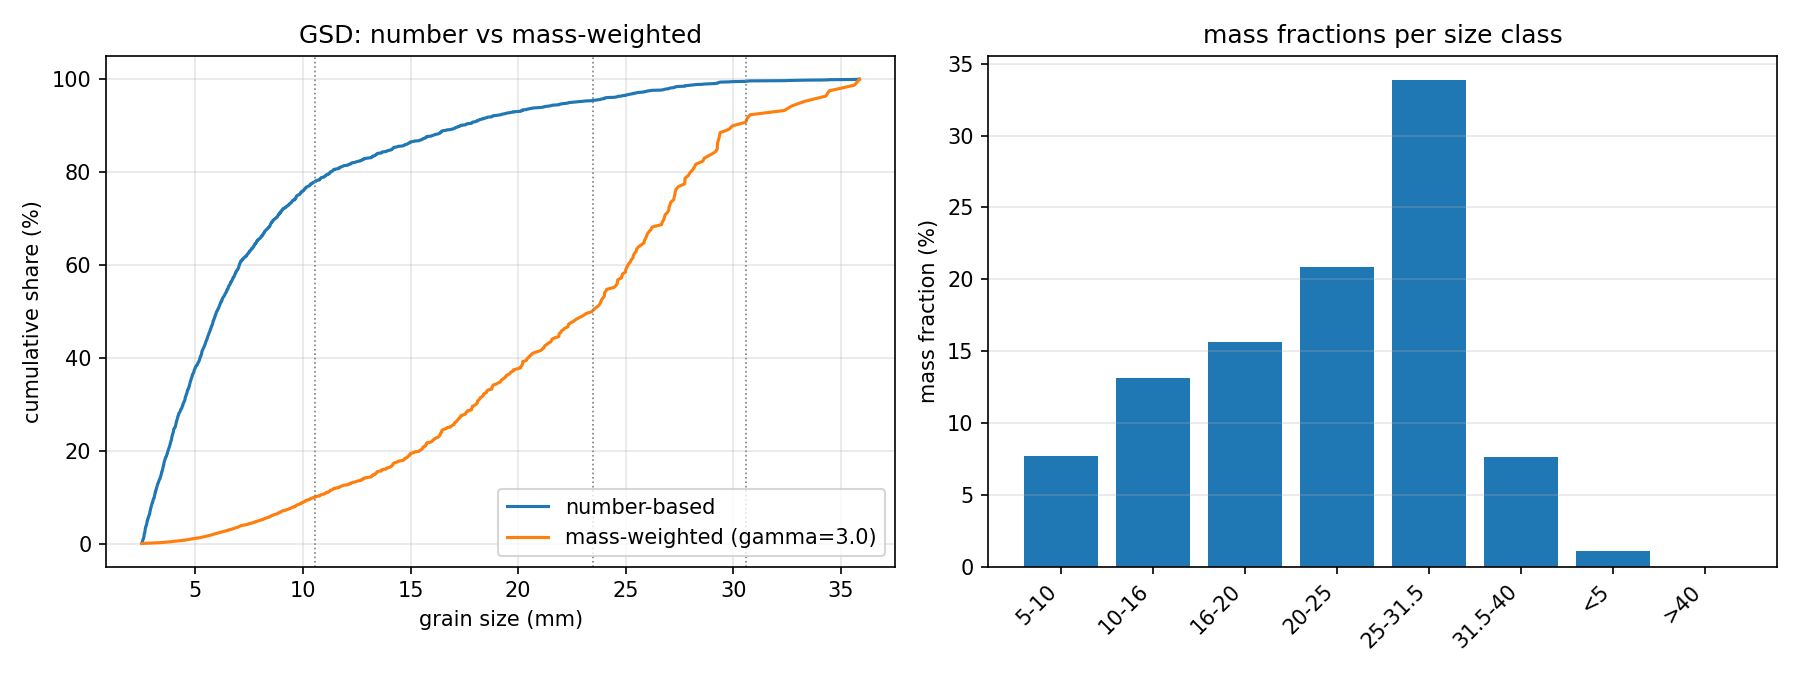
\includegraphics[width=\linewidth,height=2.6cm,keepaspectratio]{agg_001_IG2_full_set_cp_SAM_pred_grains_re_scaled_gsd_comparison.png}\\{\scriptsize 中值：$D_{50}=23.6$}\end{column}
\begin{column}{0.32\textwidth}\centering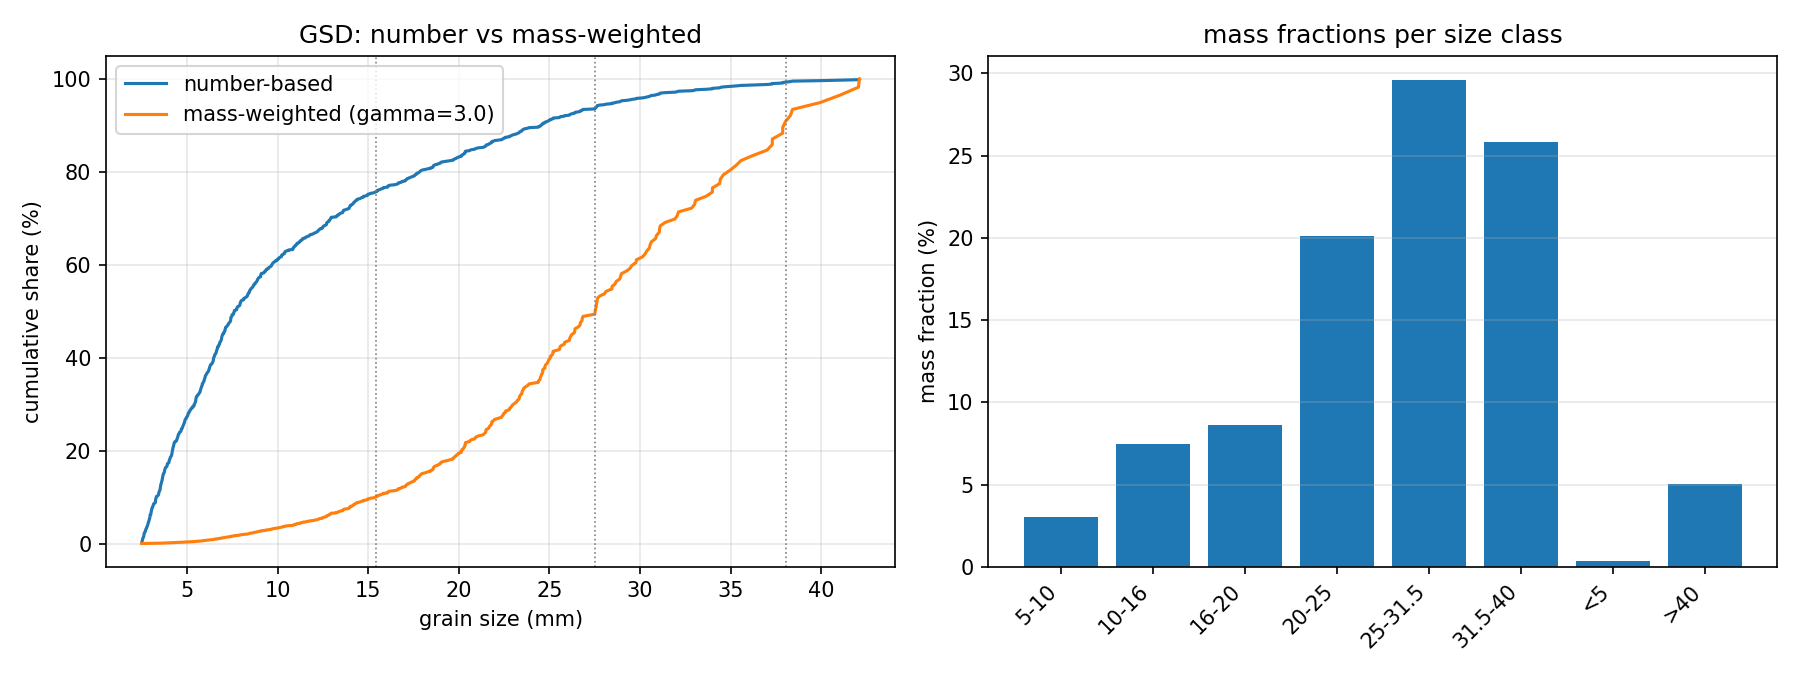
\includegraphics[width=\linewidth,height=2.6cm,keepaspectratio]{agg_005_IG2_full_set_cp_SAM_pred_grains_re_scaled_gsd_comparison.png}\\{\scriptsize 粗粒：$D_{50}=27.5$}\end{column}
\end{columns}
\vspace{0.3em}{\scriptsize\textbf{性能}：分割 $17$\,s/张 + 测量 $9$\,s，筛分 $<1$\,s；\textbf{测试}：\texttt{pytest} 27 passed（合成数据可恢复真参数）。}
\end{frame}

\section{设备与 SOP}

\begin{frame}{设备与 30\,min 现场 SOP}
\begin{columns}[T]
\begin{column}{0.52\textwidth}
{\scriptsize
\begin{tabular}{ll}
\toprule 类别 & 型号／参数 \\
\midrule
相机 & $\ge12$\,MP，$3024\times4032$ \\
标定 & 标尺／ArUco $30$\,mm \\
托盘 & 深色哑光 $60\times40$\,cm \\
光源 & 环形漫射 5000\,K \\
计算 & RTX 4080 SUPER，CUDA \\
\bottomrule
\end{tabular}}
\vspace{0.4em}
\begin{block}{一键命令}
{\scriptsize
\texttt{python -m imagegrains --img\_dir} {\small <图像>} \texttt{--resolution 0.208 --gpu True}\\
\texttt{python -m aggregate\_screening --grains *\_re\_scaled.csv --out\_dir report}}
\end{block}
\end{column}
\begin{column}{0.48\textwidth}
\textbf{30\,min SOP}
\begin{enumerate}\footnotesize
\item 摆拍 5\,min：单层＋标尺
\item 拍照 1\,min：正俯 1--3 张
\item 分割 5\,min：目检 \texttt{*\_composite.png}
\item 筛分 1\,min：出 11 件产物
\item 核对 2\,min：读 \texttt{*\_report.txt} $D$ 值
\end{enumerate}
\vspace{0.4em}{\scriptsize\color{gray}{详见 \texttt{docs/USAGE.md} 第10节，\texttt{demo\_data/samples/demo} 可复现。}}
\end{column}
\end{columns}
\end{frame}

\section{总结}

\begin{frame}{结论与展望}
\begin{columns}[T]
\begin{column}{0.58\textwidth}
\begin{itemize}\small
\item \textbf{创新}：质量加权校准链（$d,w$）\mbox{解决数量$\to$质量语义鸿沟}
\item \textbf{落地}：两步 CLI + 11 产物 + 8 可视化，30\,min 可用
\item \textbf{验证}：3 样本细／中／粗 + $\gamma$/$\theta$ 消融 + 27 测试
\end{itemize}
\vspace{0.4em}
\begin{block}{局限 $\to$ 下一步}
\footnotesize 基线 $\theta/\gamma$ $\to$ $\ge5$ 批筛分校准；标尺 $\to$ \mbox{ArUco+单应}；\mbox{几何泥团} $\to$ 裁剪分类器；CLI $\to$ 一键图形界面
\end{block}
\end{column}
\begin{column}{0.42\textwidth}
{\small\textbf{提交物}}
\begin{itemize}\scriptsize
\item 技术报告（本报告 20 页）
\item 答辩 PPT（本件 12 页）
\item 代码框架（\texttt{src/aggregate\_screening} 6 模块）
\item 设备参数（本页表）
\item 可视化辅证（11 件／样本）
\end{itemize}
\end{column}
\end{columns}
\end{frame}

\begin{frame}
\begin{center}
{\Large 谢谢！}\\[0.8em]
{\small 技术报告：\texttt{docs/paper/main.pdf}（20 页）}\\
{\small 使用手册：\texttt{docs/USAGE.md}}\\
{\small 代码：\texttt{src/aggregate\_screening/}}\\
\vspace{1em}{\scriptsize\textcolor{gray}{匿名评审，请勿含学校／导师信息}}
\end{center}
\end{frame}

\end{document}
